\documentclass[10pt]{article}

\usepackage{spheric}
%%%TITLE
\title{GPU-based SPH modeling of flood with floating bodies in urban layouts including underground spaces}
\date{}

%%AFFILIATIONS
\author[1]{Jiansong Wu$^\dagger$}
\author[1]{Na Li}
\author[1]{Wenyu Liu}
\author[2]{Hui Zhang}
\affil[1]{School of Resources and Safety Engineering, China University of Mining \& Technology, Beijing 100083, China}
\affil[2]{Institute for Public Safety Research, Tsinghua University, Beijing 10083, China}
\affil[$\relax$]{\email{\dagger}{jiansongwu@hotmail.com}}


%%DOCUMENT
\begin{document}

\maketitle

%\SelectedTopics{}

%%PLEASE PUT YOUR ABSTRACT HERE
\begin{abstract}
Due to the ``innate'' low-lying weakness, underground facilities in urban areas are prone to flooding caused by the breaking of a dam or a levee, or a flash flood after an exceptional rainfall. The underground inundation may cause loss of life and very serious damage to properties. Therefore, it is very important to study the urban underground inundation in terms of hydraulic analysis and disaster prevention. An important way of clarifying the physical phenomena and determining the risk of the underground flooding flow is to numerically simulate the inundation process.

In this paper, the mesh-free Smoothed Particle Hydrodynamics (SPH) method with the Graphic Processing Unit (GPU) parallel computing technique employed (GPUSPH) is employed to investigate dam-break flooding in complex urban underground spaces. SPH explicitly conserves mass and linear momentum, and does not require explicit interface tracking treatment so that geometrically complex and moving boundaries can be handled without undue difficulty. Taking advantage of powerful GPU parallel computing ability, the following two urban flood cases involving in millions of particles (computational nodes) are simulated: i) dam-break flood with floating bodies through an intricate surface city layouts, ii) dam-break flooding immersed three floating objects into an underground facility through staircases. Numerical results fairly reproduce the complex inundation process, and reasonably present complicated underground flooding flow features involving in interactions of flooding flow with floating objects and staircases, which indicates that SPH method is an alternative tool for the modeling of flooding in complex urban underground spaces.

\begin{figure}[!htb]
\centering
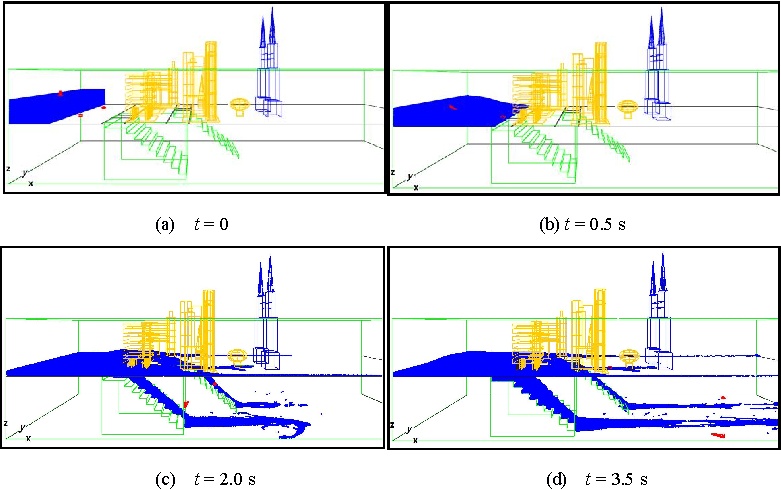
\includegraphics[width=0.85\textwidth]{26-1.pdf}
\caption{Displacement of underground flooding flow with floating objects}\label{fig:26}
\end{figure}

\end{abstract}


%%THE END OF ABSTRACT

\addbib

\end{document}
